\subsection{Euler's Critical Load Analysis}

Even though the main goal is to keep the drill string completely in tension, it is not possible to predict how much WOB that will be required to drill through the formation and it might therefore be required to increase the WOB above the limit defined in section . To set an absolute upper limit of WOB, Euler's equation (\ref{eq:eulerbuckling}) for critical load will be used. This will enable the estimation of the maximum load the pipe can bear without experiencing lateral deflection.

\begin{equation}
\centering
   F_{cr}=\frac{\pi^2 E I}{(KL)^2}
\label{eq:eulerbuckling}
\end{equation}

where $F_{cr}$ is the critical compression load (N) on the drill pipe, $E$ is the modulus of elasticity of pipe material (Pa), $I$ is the minimum area moment of inertia of the cross section of the pipe (m$^4$) given by equation (\ref{eq:momentinertia}), $L$ is the unsupported length of the pipe (m) and $K$ is the effective length factor determined by the end conditions of the pipe given in figure (\ref{fig:endcondpipe}).

\begin{equation}
\centering
   I=\frac{\pi}{64} (d_o^4-d_i^4)
\label{eq:momentinertia}
\end{equation}

where $d_o$ and $d_i$ is the outer and inner diameter of the pipe respectively.

\begin{figure} [H]
\centering
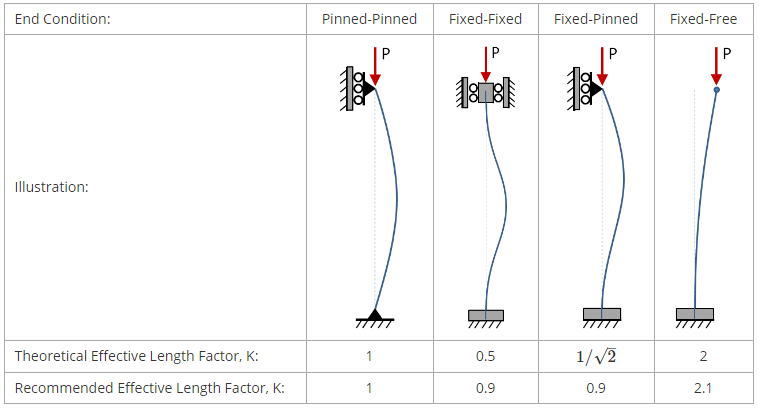
\includegraphics[width=1.0\textwidth]{figures/endcondpipe.PNG}
\caption{End conditions of pipe \cite{buckling}}
\label{fig:endcondpipe}
\end{figure}

Due to the implementation of a riser above the formation, the end conditions will be \textit{fixed-fixed}, which yields a recommended effective length factor, $K$, of 0.9.

Input data for equation (\ref{eq:eulerbuckling}) can be found in table (\ref{tab:inputdataeuler})


\begin{table} [H]
    \centering
    \caption{Input data for Euler's Critcal Load}
    \begin{tabular}{p{2cm} p{3cm}}
        E [Pa] & $6.9\cdot10^{10}$ \\ \hline
        I [m$^4$] & $2.27\cdot10^{-10}$ \\ \hline
        K & $0.9$ \\ \hline
        L [m] & $0.91$ \\ 
    \end{tabular}
    \label{tab:inputdataeuler}
\end{table}

The critical load was found to be 230.7 N, equivalent to a weight of 23.5 kg. This means that when the internal pressure is increased using the nozzle in the BHA, the pipe will enter a state of compression when the WOB passes 31.0 kg, but it will not, based on this estimation buckle until it reaches the sum of F$_c$, the drill string weight and the critical load, in this case 50 kg.

The goal will still be to avoid putting the string in compression, but if it becomes clear during phase II that a WOB of 31.0 kg is insufficient to drill efficiently, it will be considered whether a higher WOB can be used or not.